\chapter{Operators for reasoning}

It surprises me that for roughly 2222 years, logic had to be argued 
in poetic terms called syllogisms.  
\begin{quote}
    All men are mortal.\\
    Socrates is a man;\\
    Therefore Socrates is mortal.
\end{quote}
There were sing-song patterns 
to be hummed by monks. The AEIO types and the Barbara, Barbari...  
syllogistic verses.
Can you imagine writing computer programs this way?
% Syllogisms do have their place in our current reasoning,
% though admittedly more sterile.
% \begin{quote}
%     If x is a man then x is mortal.\\
%     Socrates is a man;\\
%     Therefore Socrates is mortal.
% \end{quote}

\section{Boolean algebra}\index{Boolean algebra}
Enter
George Boole and Augustus De Morgan in the 1800's to replace 
this all with algebra.  Propositions---sentences that made a 
claim we might judge to be true, were 
were reduced to symbols $P,Q,R,\ldots$
to be assigned values of true $\top$ or false $\bot$. 
Instead of meaning, logic would proceed by an assembly of 
operators $\wedge$ (and), $\vee$ (or), $\neg$ (not), and $\Rightarrow$ (implies):
\begin{gather*}
    \begin{array}{|c|c|}
        \hline 
         & \neg \\
        \hline 
        \top & \bot \\
        \bot & \top\\
        \hline
    \end{array}
    \qquad
    \begin{array}{|c|cc|}
        \hline 
        \wedge & \top & \bot\\
        \hline 
        \top & \top & \bot \\
        \bot & \bot & \bot\\
        \hline
    \end{array}
    \qquad 
    \begin{array}{|c|cc|}
        \hline 
        \vee & \top & \bot\\
        \hline 
        \top & \top & \top \\
        \bot & \top & \bot\\
        \hline
    \end{array}
    \qquad
    \begin{array}{|c|cc|}
        \hline 
        \Rightarrow & \top & \bot\\
        \hline 
        \top & \top & \bot \\
        \bot & \top & \top\\
        \hline
    \end{array}
\end{gather*}
Today this is called \emph{Boolean algebra}, but De Morgan's laws 
are also taught to those who reason.

\index{Symbolic Logic}
Reasoning based solely on truth values never quite won out.
For one thing, sometimes we need to reason solely about the argument, not the content.
\begin{quote}
    All Pok\'emon are immortal; \\
    Pikachu is a Pok\'emon;\\
    therefore Pikachu is immortal.
\end{quote}
It is difficult to assign this sentence any truth value since 
the subject is fantasy of a Pok\'emon species.  
Even so it seems the same form as our prior syllogism.
John Venn supplied the option to instead operate on symbols:
\begin{center}
\begin{minipage}{0.45\textwidth}
\begin{gather}
    \tag{Modus Ponens}
    \begin{array}{crl}
       &  P &\Rightarrow Q\\
     \wedge  &  P\\
    \hline 
       &  Q
    \end{array}
\end{gather}
\end{minipage}
\hfill
\begin{minipage}{0.45\textwidth}
    \begin{gather}
        \tag{Variable Arithmetic}
        \begin{array}{crl}
           &  x & + y\\
         -  &  x\\
        \hline 
            &  y
        \end{array}
    \end{gather}
\end{minipage}        
\end{center}
Notice this is a modest departure from operators we invent to 
work with polynomials.  Venn's name lives on with his 
diagram language, the algebra he suggested is known variously 
as \emph{Symbolic, Syntatic,} or \emph{Formal} Logic.  (Formal here means 
having to do with form, it does not mean a logic fit for fine dining.)

\section{Judgement Operators}
Venn's logic brought Boolean rigor to variable content but still focussed 
on method not meaning.  Gottlob Frege added the back the meaning of arguments
(semantics ) with two further operators:
\begin{itemize}
    \item $|P$ \emph{Urteilsstrich} (judgement bar), written to pass judgement 
    on $P$.  As is common writing $|P$ alone abbreviates saying $|P=\top$, i.e.\
     ``$P$ is true''.  To say ``$P$ is false'' we may write $|P=\bot$ or $\not| P$.

    \item $-P$ \emph{Inhaltsstrich} (content bar), written to shift reasoning 
    to the content of $P$, e.g.\ Socrates and Pok\'emon, rather than the 
    form of the sentence.
\end{itemize}
Strictly speaking $|-P$ is an operation on $P$, to pass judgement on its content.
Yet, we try not to publish things known to be false so we have little need for 
writing ``$|-P=\bot$'', preferring to write $|- (\not P)=\top$ (``not P is true'').
This leaves us the default assumption that when we bother to 
judge $P$ it is because it will be true.  So it is accepted practice to have:
\begin{center}
    $|-P$ read as ``The content of $P$ is true.'' 
\end{center}
So common is this today that the two operators are fused into one
``turnstyle'' character $\vdash P$.  When we judge $P$ in the presence of 
other propositions $P_1,\ldots, P_n$, then we simply prepend these conditions before the turnstyle 
using anyone one of the following interchangeable notations.
\begin{gather*}
    P_1,\ldots,P_n\vdash P 
    \qquad 
    \frac{P_1,\ldots,P_n}{P}
    \qquad 
    \begin{array}{c}
        P_1\\ \vdots \\ P_n\\ \hline P 
    \end{array}
\end{gather*}
The astute reader will recognize this makes $\vdash$ into a variadic operator.\index{variadic}
One remedy for this is to group lists into a single ``multiset'' (intentionally leaving 
that concept intuitive and imprecise) $\Gamma$ and write $\Gamma\vdash P$ so that we have a 
simple bivalent operator instead.

\section{Intuitionistic Operators}
Similar to Boolean algebra, there are today a various natural operators on Frege styled 
syntatic an semantic reasoning.  Here for example is a minimal list meant to express 
what is known as \emph{intuitionistic} logic.  We first show the rule, or rules, that introduce
the operator, and then the rule(s) that use is, that is eliminate the symbol of the operator.
We start with the Modus Ponens from above.  Throughout we let $\Gamma$ be all the assumptions 
made in the context of our problem.

\subsection{Implication $\Rightarrow$}
If context $\Gamma$ or context together with $P$ can prove $Q$ then context 
can prove $P\Rightarrow Q$:
\begin{align*}
    \frac{\Gamma\vdash Q}{\Gamma\vdash P\Rightarrow Q}(\intro{\Rightarrow})
    \qquad 
    \frac{\Gamma,P\vdash Q}{\Gamma \vdash P\Rightarrow Q}(\intro{\Rightarrow})
\end{align*}
Notice a material difference in this implication and that of Boole.  Here there is 
no concept of ``false implying true''.  While we still support $Q$ being true without 
$P$ necessarily true (the left-hand introduction), we still depend on context $\Gamma$ 
to claim that $Q$ is true.  

Once we have an implication and the premise, we get to use it to eliminate the symbol 
$\Rightarrow$.
\begin{gather}
    \tag{$\elim{\Rightarrow}$}
    \begin{array}{rrl}
       \Gamma &\vdash  P &\Rightarrow Q\\
     \Delta  &\vdash  P\\
    \hline 
      \Gamma,\Delta &\vdash  Q
    \end{array}
\end{gather}

\subsection{And $\wedge$}

Conjunction says two trues can be combined as one.
\begin{align*}
    \tag{$\intro{\wedge}$}
    \begin{array}{rl}
        \Gamma & \vdash P\\
        \Delta & \vdash Q\\
    \hline 
        \Gamma,\Delta & \vdash P\wedge Q
    \end{array}
\end{align*}
From a conjoined truth we can retrieve individual truths.
\begin{align*}
    \tag{$\elim{\wedge}$}
    \frac{\Gamma\vdash P\wedge Q}{\Gamma\vdash P}
    \qquad 
    \frac{\Gamma\vdash P\wedge Q}{\Gamma\vdash Q}
\end{align*}
We can diagram this as a comic strip.  The introduction followed by the 
elimination.
\begin{center}
    \begin{tikzpicture}
        \node (form) {\begin{tikzpicture}
            \coordinate (Gp) at (0,1);
            \coordinate (Dp) at (0,-1);
            % \coordinate (GDp) at (0,0);
            \coordinate (Pp) at (2,1);
            \coordinate (Qp) at (2,-1);
            % \coordinate (PQp) at (2,0);

            % \fill[black!10] (Gp.west) -- (Pp) -- (Qp.south east) -- (Dp) -- cycle;

            \node (G) at (Gp) {$\Gamma$};
            % \node (GD) at (GDp) {$\Gamma,\Delta$};
            \node (D) at (Dp) {$\Delta$};
            \node (P) at (Pp) {$P$};
            \node (Q) at (Qp) {$Q$};
            % \node (PQ) at (PQp) {$P\wedge Q$};
            \draw[|-] (G) -- (P);
            \draw[|-] (D) -- (Q);
            % \draw[|-] (GD) -- (PQ);
            % \draw[|-] (GD) -- (G);
            % \draw[|-] (GD) -- (D);
            % \draw[|-] (PQ) -- (P);
            % \draw[|-] (PQ) -- (Q);
        \end{tikzpicture}};
        \draw[thick,-] (form.north west) -- (form.south west);

        \node (intro) at ($(form.east)+(2,0)$) {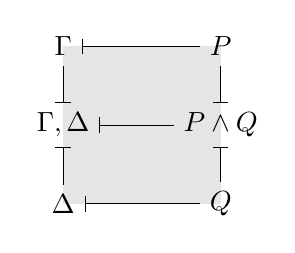
\begin{tikzpicture}
            \coordinate (Gp) at (0,1);
            \coordinate (Dp) at (0,-1);
            \coordinate (GDp) at (0,0);
            \coordinate (Pp) at (2,1);
            \coordinate (Qp) at (2,-1);
            \coordinate (PQp) at (2,0);

            \fill[black!10] (Gp.west) -- (Pp) -- (Qp.south east) -- (Dp) -- cycle;

            \node (G) at (Gp) {$\Gamma$};
            \node (GD) at (GDp) {$\Gamma,\Delta$};
            \node (D) at (Dp) {$\Delta$};
            \node (P) at (Pp) {$P$};
            \node (Q) at (Qp) {$Q$};
            \node (PQ) at (PQp) {$P\wedge Q$};
            \draw[|-] (G) -- (P);
            \draw[|-] (D) -- (Q);
            \draw[|-] (GD) -- (PQ);
            \draw[|-] (GD) -- (G);
            \draw[|-] (GD) -- (D);
            \draw[|-] (PQ) -- (P);
            \draw[|-] (PQ) -- (Q);

        \end{tikzpicture}};
        \draw[thick,-] (intro.north west) -- (intro.south west);
    \end{tikzpicture}
\end{center}
We will often include such comics as they lead to diagrams between 
data and eventually also diagrams in allegories and categories.

\subsection{Falsity $\bot$}
While truth may be easy to judge, we are less certain about what is false as 
G\"odel and Turing taught us to prepare for a future with unknowables as well.
So to claim something is false is a stronger claim than to claim something 
is untrue.
False therefore shall mean something that can lead to any other conclusion.
\begin{align}
    \tag{$\elim{\bot}$}
    \frac{\Gamma\vdash \bot}{\Gamma\vdash P}
\end{align}
Notice we did not give a means to introduce falsity and that is because we 
are engaged in writing down only truths.  So if we want to create a falsity 
we must do so through an indirect path such as implication.  Here is an example.
\begin{align}
    \tag{Proof by negation}
    \begin{array}{rl}
    \Gamma & \vdash P\Rightarrow \bot \\
    \Delta & \vdash P \\
    \hline 
    \Gamma,\Delta & \vdash \bot
    \end{array}
\end{align}
Engaging in some provocative notation we can define 
\begin{align*}
    \neg P \defeq (P\Rightarrow \bot)
\end{align*}
In this way proof by negation says 
\begin{align*}
    \frac{(\neg P)\wedge P}{\bot}.
\end{align*}
This is all notation and there really is not false becoming true.  Notice 
if $P$ is neither true nor false then we will never succeed in making 
$(\neg P)$ and $P$ at the same time.  So this allows us to face the reality 
of such systems.  While it is safe to make an axioms that declares all 
propositions are true or false (Law of the Excluded Middle) there are natural 
systems in algebra, topology, and computation that simply do not obey that law 
so it is best to avoid it until required.

% \section{Heyting algebra}
